%%%%%%%%%%%%%%%%%%%%%%%%%%%%%%%%%%%%%%%%%%%%%%%%%
% Chapter: Data Access Operations
%%%%%%%%%%%%%%%%%%%%%%%%%%%%%%%%%%%%%%%%%%%%%%%%%
\chapter{Data Access and Sharing}
\label{chap:data_sharing}

In \ac{PMIx} key-value pairs are the primary way that information is shared 
between processes in the \ac{PMIx} universe.  
A key-value pair consists of a string key and a value data structure
which includes the type of the value's data.  
Each key is unique within the context or domain in which it exists.
The context or domain of a key in PMIx is called a data realm.  
%% The pmix_info_t type (See \ref{chap:introduction:portability:attributes}), 
%% is also built on key-values pairs.  
%% However, pmix_info_t is used for influencing API calls and is not used for sharing 
%% information between processes.  
This chapter describes how key-value pairs are made available and accessed by clients.

A key-value pair has a scope defined by its data realm.  
PMIx defines data realms for sessions, jobs, applications, nodes, processes and a special 
realm for publish/lookup information.   
These are explained more fully in chapters \ref{chap:api_rsvd_keys} and \ref{chap:pub}.

The source or provider of key-value pairs can be the host environment or a \ac{PMIx} client.  
The host environment can provide key-values pairs in any realm except for the publish/lookup realm.
%%% Can we have a separate effort to change this restriction on publish/lookup for consistency?
%%% Would this get into too many other issues?
PMIx clients can only provide key-values pairs within their own process realm and the publish/lookup realm.
The value of a key is not necessarily static and can be modified by the original provider of the key.

\ac{PMIx} classifies keys as either reserved or non-reserved.

Only keys provided by a host environment or \ac{PMIx} implementation can begin with \code{"pmix"} and are called reserved keys.  
Host environments and \ac{PMIx} implementations must only provide keys that begin with \code{"pmix"} to avoid conflicts with keys that are provided by clients.
Reserved keys are documented in chapter \ref{chap:api_rsvd_keys}.
Each standardized reserved key has an associated macro that is documented along with its description.
Likewise clients can only provide keys that do not begin with \code{"pmix"} to avoid conflicting with keys provided by the host environment or \ac{PMIx} implementation.   
The string representation and the macro are equivalent methods to refer to a key.
Throughout this document, the macro is used rather than its string value to refer to reserved keys.
Clients cannot create reserved keys, nor can they modify the value of reserved keys.
The way reserved keys are accessed by clients 
is different than for non-reserved keys as explained in \ref{chap:api_rsvd_keys}.

Host environments are not required to provide all keys that are documented in the standard.  
However, when providing keys that are documented, they must adhere to the behavior defined by the standard for reserved keys.  
An implementation cannot provide a reserved key that behaves differently than what is in the standard.  
Implementations are encouraged to standardize any non-standardized, reserved keys that they provide to avoid conflicting with other implementations or efforts to standardize the same key.

Host environments are permitted to provide non-reserved keys and non-standardized reserved keys.  
However there are important caveats to providing either of these categories of keys 
that are explained in \ref{chap:data_sharing:non_rsvd_keys} and \ref{chap:api_rsvd_keys}.
% Would like to make this statement stronger, but there is text in chapter 6 currently that
% says it is allowed to use "custom-prefixed keys which may adhere to either the reserved or non-reserved
% retrieval rules.
Host environments should avoid providing reserved keys which are not standardized.  
If the reserved key is later standardized to behave in a way that is different from the behavior 
provided by the host environment, the host environment will not be compliant with the PMIx standard.
 
Reserved keys are set by the host environment and are made available at client initialization. 
Each key is associated with a data realm and the retrieval API call will indicate the realm being queried.
Reserved keys are used to access information about a client's execution context.
After initialization, the client can access reserved keys using the PMIx_Get API.  
Common information that a client may access includes, but is not limited to,
the name of the host it is executing on, 
the number of peer processes in its namespace,
the number of peer processes in its application,
and its job rank.

%%% (Do we want to make any other statements about how and when values can change during 
%%%  the course of execution.
%%%  PMIX_EXIT_CODE for example, UNIVERSE_SIZE could change if more resources are added?)

Non-reserved keys are provided by clients.
A call to PMIx_Put will result in a key-value being associated with the calling client within 
its process data realm.
There is no mechanism to retract a key-value that has been made available by a client through \refapi{PMIx_Put}.
The key can be assigned a new value, but cannot be removed entirely.
Although key values can originate from different sources, they are always retrieved using the
\refapi{PMIx_Get} and \refapi{PMIx_Get_nb} API.

The publish/lookup data realm is accessed through a separate set of API's.
\refapi{PMIx_Put} cannot add or modify key-values within the publish/lookup realm and 
\refapi{PMIx_Lookup} cannot access key-values outside the publish/lookup realm.
This data realm is described in detail is chapter [Reference to publish/lookup chapter].
Although PMIx_Publish and PMIx_Lookup are analogous to PMIx_Put and PMIx_Get in that both pairs 
of API's provide functionality for exposing and retreiving key-values, the semantics vary significantly.  
For example, PMIx_Lookup includes the ability to wait until a key is defined before returning.
PMIx_Publish can restrict the scope of who can access data to its own namespace, the host environment, the session it is executing in, all processes or even custom scopes, while  
PMIx_Put can restrict the scope of who can access data to the node it is executing on, remote nodes, 
all nodes or only itself.
The publish/lookup data realm is useful for advertising information that is not necessarily specific to one process to other processes in the \ac{PMIx} universe.
The process accessing this information does \emph{not} need to know the identity of the process that provided the data.

\ac{PMIx} does not provide a mechanism to asynchronously notify a process about the availability of key-value information once it is made available by another process.
However, the nonblocking accessor interfaces (e.g., \refapi{PMIx_Get_nb}, \refapi{PMIx_Lookup_nb}) may provide a degree of asynchronous notification on information availability.

Process related key-value exchanges allow a \ac{PMIx} process to share information specific to 
itself, and access information specific to one or more processes in the \ac{PMIx} universe.
These interactions occur within the process data realm.
The 'put/commit/get' exchange pattern is often used to exchange process related information.
Optionally, a 'put/commit/fence/get' exchange pattern adds the 'fence' synchronization 
(and possible collective exchange) for applications that desire it.
Commonly, these exchange patterns are used in a 
\declareterm{business card exchange} (a.k.a. \declareterm{modex exchange}) 
where one \ac{PMIx} client shares its connectivity information, then other \ac{PMIx} clients access that information to establish a connection with that client.
In some environments that support ``instant-on'' all connectivity information for \ac{PMIx} clients is stored in the job-level information at process creation time and is accessible to the clients without the need to perform any additional key-value exchange.

Keys can exist in multiple data realms, possibly with different values. 
\ac{PMIx} clients can access available information associated with any of the data realms.
For example, a client can access the number of nodes (\refattr{PMIX_NUM_NODES}) used by a 
session, job, or application.
Rather than having three different attributes, a single attribute is used but with the 
data realm context of the query specified as additional attributes.
Examples of these access patterns are presented in Section \ref{chap:api_rsvd_keys:getex}.

\ac{PMIx} clients can share key-value pairs associated with themselves by using the \refapi{PMIx_Put} function.
The \refapi{PMIx_Put} function automatically associates the key-value pair with the calling process, thus making it specific to that process.
A client may call \refapi{PMIx_Put} as many times as necessary and the data is not available to other processes until explicitly committed.
A client must call \refapi{PMIx_Commit} to make accessible all key-value pairs previously put by this process to all other processes in the \ac{PMIx} universe.
This put and commit pattern provides implementors the opportunity to make individual \refapi{PMIx_Put} calls efficient local operations, and then make the whole set of key-value pairs accessible in a single step.

\ac{PMIx} clients can access the key-value pairs associated with any process data realm 
in the \ac{PMIx} universe (including the calling process) by passing the specific process 
name of the target process to the \refapi{PMIx_Get} and \refapi{PMIx_Get_nb} functions.
The \ac{PMIx} server local to the calling process will retrieve that key-value pair from 
the \ac{PMIx} server associated with the target process.
Clients can also access session, job, application, node, and namespace level information 
by using the \refapi{PMIx_Get} and \refapi{PMIx_Get_nb} functions as shown in Section 
\ref{chap:api_rsvd_keys:getex}.
% and summarized in Table~\ref{tab:key-value-realms}.  (Add in next release?)
The completion semantics for \refapi{PMIx_Get} and \refapi{PMIx_Get_nb} differ 
depending on the type of key and its availability.  See Sections 
\ref{chap:data_sharing:retrules} and \ref{chap:api_rsvd_keys:retrules}.
For example, if a non-reserved key is not available, the \refapi{PMIx_Get} or \refapi{PMIx_Get_nb} call 
will not complete, by default, until that key-value pair becomes available.

%%%%%%%%%%%%%%%%%%%%%%%%%%%%%%%%%%%%%%%%%%%%%%%%%
\section{Non-reserved keys}
\label{chap:data_sharing:non_rsvd_keys}

\emph{Non-reserved keys} are keys whose string representation begin with a
prefix other than \code{"pmix"}. Such keys are defined by a
client when information needs to be exchanged between processes, for example, 
where connection information is required and the host environment does not
support the \refterm{instant on} option) or where the host environment does not
provide a required piece of data. Other than the prefix, there are no
restrictions on the use or content of non-reserved keys.

\ac{PMIx} provides support for two methods of exchanging non-reserved keys:

\begin{itemize}
    \item Global, collective exchange of the information prior to retrieval. This is accomplished by executing a barrier operation that includes collection and exchange of the data provided by each process such that each process has access to the full set of data from all participants once the operation has completed. \ac{PMIx} provides the \refapi{PMIx_Fence} function (or its non-blocking equivalent) for this purpose, accompanied by the \refattr{PMIX_COLLECT_DATA} qualifier.
    \item Direct, on-demand retrieval of the information. No barrier or global exchange is conducted in this case. Instead, information is retrieved from the host where that process is executing upon request - i.e., a call to \refapi{PMIx_Get} results in a data exchange with the \ac{PMIx} server on the remote host. Various caching strategies may be employed by the host environment and/or \ac{PMIx} implementation to reduce the number of retrievals. Note that this method requires that the host environment both know the location of the posting process and support direct information retrieval.
\end{itemize}

Both of the above methods are based on retrieval from a specific process -
i.e., the \refarg{proc} argument to \refapi{PMIx_Get} must include both the
namespace and the rank of the process that posted the information. However, in
some cases, non-reserved keys are provided on a globally unique basis and the
retrieving process has no knowledge of the identity of the process posting the
key. This is typically found in legacy applications (where the originating
process identifier is often embedded in the key itself) and in unstructured
applications that lack rank-related behavior. In these cases, the key remains
associated with the namespace of the process that posted it, but is retrieved
by use of the \refconst{PMIX_RANK_UNDEF} rank. In addition, the keys must be
globally exchanged prior to retrieval as there is no way for the host to
otherwise locate the source for the information.

Note that the retrieval rules for non-reserved keys (detailed in Section 
\ref{chap:data_sharing:retrules}) differ significantly from those used for reserved keys.


%%%%%%%%%%%%%%%%%%%%%%%%%%%%%%%%%%%%%%%%%%%%%%%%%
%%%%%%%%%%%%%%%%%%%%%%%%%%%%%%%%%%%%%%%%%%%%%%%%%
\section{Posting Key/Value Pairs}
\label{chap:data_sharing:set}

\ac{PMIx} clients can post non-reserved key-value pairs associated with themselves by using \refapi{PMIx_Put}. Alternatively, \ac{PMIx} clients can cache both reserved and non-reserved key-value pairs accessible only by the caller via the \refapi{PMIx_Store_internal} \ac{API}.


%%%%%%%%%%%%%%%%%%%%%%%%%%%%%%%%%%%%%%%%%%%%%%%%%
\subsection{\code{PMIx_Put}}
\declareapi{PMIx_Put}

%%%%
\summary

Stage a key/value pair in prepartion for being made accessible to processes.

%%%%
\format

\versionMarker{1.0}
\cspecificstart
\begin{codepar}
pmix_status_t
PMIx_Put(pmix_scope_t scope,
         const pmix_key_t key,
         pmix_value_t *val);
\end{codepar}
\cspecificend

\begin{arglist}
\argin{scope}{Distribution scope of the provided value (handle)}
\argin{key}{key (\refstruct{pmix_key_t})}
\argin{value}{Reference to a \refstruct{pmix_value_t} structure (handle)}
\end{arglist}

Returns \refconst{PMIX_SUCCESS} or a negative value corresponding to a \ac{PMIx} error constant.
If a reserved key is provided in the \refarg{key} argument then \refapi{PMIx_Put} will return \refconst{PMIX_ERR_BAD_PARAM}.

%%%%
\descr

Post a key-value pair for distribution. Depending upon the \ac{PMIx} implementation, the posted value may be locally cached in the client's \ac{PMIx} library until \refapi{PMIx_Commit} is called.

The provided \refarg{scope} determines the ability of other processes to access the posted data, as defined in \specrefstruct{pmix_scope_t}.
Specific implementations may support different scope values, but all implementations must support at least \refconst{PMIX_GLOBAL}.

The \refstruct{pmix_value_t} structure supports both string and binary values.
\ac{PMIx} implementations are required to support heterogeneous environments by properly converting binary values between host architectures, and will copy the provided \refarg{value} into internal memory prior to returning from \refapi{PMIx_Put}.

\adviceuserstart
Note that keys starting with a string of ``\code{pmix}'' must not be used in calls to \refapi{PMIx_Put}. Thus, applications should never use a defined ``PMIX'' attribute as the key in a call to \refapi{PMIx_Put}.
\adviceuserend


%%%%%%%%%%%%%%%%%%%%%%%%%%%%%%%%%%%%%%%%%%%%%%%%%
\subsubsection{Scope of Put Data}
\declarestruct{pmix_scope_t}
\label{api:nres:scope}

\versionMarker{1.0}
The \refstruct{pmix_scope_t} structure is a \code{uint8_t} type that defines the availability of data passed to \refapi{PMIx_Put}.
The following constants can be used to set a variable of the type \refstruct{pmix_scope_t}. All definitions were introduced in version 1 of the standard unless otherwise marked.

Specific implementations may support different scope values, but all implementations must support at least \refconst{PMIX_GLOBAL}.
If a specified scope value is not supported, then the \refapi{PMIx_Put} call must return \refconst{PMIX_ERR_NOT_SUPPORTED}.

\begin{constantdesc}
%
\declareconstitem{PMIX_SCOPE_UNDEF}
Undefined scope.
%
\declareconstitem{PMIX_LOCAL}
The data is intended only for other application processes on the same node.
Data marked in this way will not be included in data packages sent to remote requesters - i.e., it is only available to processes on the local node.
%
\declareconstitem{PMIX_REMOTE}
The data is intended solely for applications processes on remote nodes.
Data marked in this way will not be shared with other processes on the same node - i.e., it is only available to  processes on remote nodes.
%
\declareconstitem{PMIX_GLOBAL}
The data is to be shared with all other requesting processes, regardless of location.
%
\versionMarker{2.0}
\declareconstitem{PMIX_INTERNAL}
The data is intended solely for this process and is not shared with other processes.
%
\end{constantdesc}


%%%%%%%%%%%%%%%%%%%%%%%%%%%%%%%%%%%%%%%%%%%%%%%%%
\subsection{\code{PMIx_Store_internal}}
\declareapi{PMIx_Store_internal}

%%%%
\summary

Store some data locally for retrieval by other areas of the process.

%%%%
\format

\versionMarker{1.0}
\cspecificstart
\begin{codepar}
pmix_status_t
PMIx_Store_internal(const pmix_proc_t *proc,
                    const pmix_key_t key,
                    pmix_value_t *val);
\end{codepar}
\cspecificend

\begin{arglist}
\argin{proc}{process reference (handle)}
\argin{key}{key to retrieve (string)}
\argin{val}{Value to store (handle)}
\end{arglist}

Returns \refconst{PMIX_SUCCESS} or a negative value corresponding to a PMIx error constant.
If a reserved key is provided in the \refarg{key} argument then \refapi{PMIx_Store_internal} will return \refconst{PMIX_ERR_BAD_PARAM}.

%%%%
\descr

Store some data locally for retrieval by other areas of the process.
This is data that has only internal scope - it will never be posted externally. Typically used to cache data obtained by means outside of \ac{PMIx} so that it can be accessed by various areas of the process.


%%%%%%%%%%%%%%%%%%%%%%%%%%%%%%%%%%%%%%%%%%%%%%%%%
\subsection{\code{PMIx_Commit}}
\declareapi{PMIx_Commit}

%%%%
\summary

Make available to other processes all key-value pairs previously staged via \refapi{PMIx_Put}.

%%%%
\format

\versionMarker{1.0}
\cspecificstart
\begin{codepar}
pmix_status_t PMIx_Commit(void);
\end{codepar}
\cspecificend

Returns \refconst{PMIX_SUCCESS} or a negative value corresponding to a PMIx error constant.

%%%%
\descr

\ac{PMIx} implementations may choose to locally cache non-reserved keys prior to submitting them for distribution.  \refapi{PMIx_Commit} initiates the operation of making available previously staged key-value pairs to other processes.  Depending on the implementation, this may involve transmitting the entire collection of data posted by the process to a server.  \refapi{PMIx_Commit} is an asynchronous operation that will immediately return to the caller while the data is staged in the background.

\adviceuserstart
Users are advised to always include the call to \refapi{PMIx_Commit} in case the local implementation requires it. Note that posted data will not be circulated during \refapi{PMIx_Commit}. Availability of the data by other processes upon completion of \refapi{PMIx_Commit} therefore still relies upon the exchange mechanisms described at the beginning of this chapter.
\adviceuserend


%%%%%%%%%%%%%%%%%%%%%%%%%%%%%%%%%%%%%%%%%%%%%%%%%
\section{Retrieval rules for non-reserved keys}
\label{chap:data_sharing:retrules}

Since non-reserved keys cannot, by definition, have been provided by the host
environment, their retrieval follows significantly different rules than those
defined for reserved keys (as detailed in Section \ref{chap:api_rsvd_keys}).
\refapi{PMIx_Get} for a non-reserved key will obey the
following precedence search:

\begin{enumerate}
    \item If the \refattr{PMIX_GET_REFRESH_CACHE} attribute is given, then the
    request is first forwarded to the local \ac{PMIx} server which will then
    update the client's cache. Note that this may not, depending upon
    implementation details, result in any action.

    \item Check the local \ac{PMIx} client cache for the requested key - if not found and either the \refattr{PMIX_OPTIONAL} or \refattr{PMIX_GET_REFRESH_CACHE} attribute was given, the search will stop at this point and return the \refconst{PMIX_ERR_NOT_FOUND} status.

    \item Request the information from the local \ac{PMIx} server. The server
    will check its cache for the specified key. If the
    value still isn't found and the \refattr{PMIX_IMMEDIATE} attribute was
    given, then the library shall return the \refconst{PMIX_ERR_NOT_FOUND}
    error constant to the requester. Otherwise, the \ac{PMIx} server library
    will take one of the following actions:
    \begin{compactitemize}
        \item If the target process has a rank of \refconst{PMIX_RANK_UNDEF},
        then this indicates that the key being requested is globally unique
        and \emph{not} associated with a specific process. In this case, the
        server shall hold the request until either the data appears at the
        server or, if given, the \refattr{PMIX_TIMEOUT} is reached. In the
        latter case, the server will return the \refconst{PMIX_ERR_TIMEOUT}
        status. Note that the server may, depending on \ac{PMIx}
        implementation, never respond if the caller failed to specify a
        \refattr{PMIX_TIMEOUT} and the requested key fails to arrive at the
        server.

        \item If the target process is \emph{local} (i.e., attached to the
        same \ac{PMIx} server), then the server will hold the request until
        either the target process provides the data or, if given, the
        \refattr{PMIX_TIMEOUT} is reached. In the latter case, the server will
        return the \refconst{PMIX_ERR_TIMEOUT} status. Note that data which is
        posted via \refapi{PMIx_Put} but not staged with \refapi{PMIx_Commit}
        may, depending upon implementation, never appear at the server.

        \item If the target process is \emph{remote} (i.e., not attached to
        the same \ac{PMIx} server), the server will either:
        \begin{compactitemize}
            \item If the host has provided the
            \refapi{pmix_server_dmodex_req_fn_t} module function
            interface, then the server
            shall pass the request to its host for servicing. The host is
            responsible for determining the location of the target process and
            passing the request to the \ac{PMIx} server at that location.

            When the remote data request is received, the target \ac{PMIx}
            server will check its cache for the specified key. If the key is
            not present, the request shall be held until either the target
            process provides the data or, if given, the \refattr{PMIX_TIMEOUT}
            is reached. In the latter case, the server will return the
            \refconst{PMIX_ERR_TIMEOUT} status. The host shall convey the
            result back to the originating \ac{PMIx} server, which will reply
            to the requesting client with the result of the request when the
            host provides it.

            Note that the target server may, depending on \ac{PMIx}
            implementation, never respond if the caller failed to specify a
            \refattr{PMIX_TIMEOUT} and the target process fails to post the
            requested key.

            \item if the host does not support the
            \refapi{pmix_server_dmodex_req_fn_t} interface, then
            the server will immediately respond to the client with the
            \refconst{PMIX_ERR_NOT_FOUND} status
        \end{compactitemize}
    \end{compactitemize}
\end{enumerate}

\adviceimplstart
While there is no requirement that all \ac{PMIx} implementations follow the
client-server paradigm used in the above description, implementers are
required to provide behaviors consistent with the described search pattern.
\adviceimplend

\adviceuserstart
Users are advised to always specify the \refattr{PMIX_TIMEOUT} value when
retrieving non-reserved keys to avoid potential deadlocks should the specified
key not become available.
\adviceuserend

%%%%%%%%%%%%%%%%%%%%%%%%%%%%%%%%%%%%%%%%%%%%%%%%%
%%%%%%%%%%%%%%%%%%%%%%%%%%%%%%%%%%%%%%%%%%%%%%%%%
\section{\code{PMIx_Get}}
\declareapi{PMIx_Get}

%%%%
\summary

Retrieve a key/value pair from the client's namespace.

%%%%
\format

\versionMarker{1.0}
\cspecificstart
\begin{codepar}
pmix_status_t
PMIx_Get(const pmix_proc_t *proc, const pmix_key_t key,
         const pmix_info_t info[], size_t ninfo,
         pmix_value_t **val);
\end{codepar}
\cspecificend

\begin{arglist}
\argin{proc}{Process identifier - a \code{NULL} value may be used in place of the caller's ID (handle)}
\argin{key}{Key to retrieve (\refstruct{pmix_key_t})}
\argin{info}{Array of info structures (array of handles)}
\argin{ninfo}{Number of elements in the \refarg{info} array (integer)}
\argout{val}{value (handle)}
\end{arglist}

A successful return indicates that the requested data has been returned in the manner requested (.e.g., in a provided static memory location ).

\returnstart
\begin{itemize}
\item \refconst{PMIX_ERR_BAD_PARAM} A bad parameter was passed to the function call - e.g., the request included the \refattr{PMIX_GET_STATIC_VALUES} directive, but the provided storage location was \code{NULL}
\item \refconst{PMIX_ERR_EXISTS_OUTSIDE_SCOPE} The requested key exists, but was posted in a \emph{scope} (see Section \ref{api:nres:scope}) that does not include the requester.
\item \refconst{PMIX_ERR_NOT_FOUND} The requested data was not available.
\end{itemize}
\returnend

\reqattrstart
The following attributes are required to be supported by all \ac{PMIx} libraries:

\pasteAttributeItem{PMIX_OPTIONAL}
\pasteAttributeItem{PMIX_IMMEDIATE}
\pasteAttributeItem{PMIX_DATA_SCOPE}
\pasteAttributeItem{PMIX_SESSION_INFO}
\pasteAttributeItem{PMIX_JOB_INFO}
\pasteAttributeItem{PMIX_APP_INFO}
\pasteAttributeItem{PMIX_NODE_INFO}
\pasteAttributeItem{PMIX_GET_STATIC_VALUES}
\pasteAttributeItem{PMIX_GET_POINTER_VALUES}
\pasteAttributeItem{PMIX_GET_REFRESH_CACHE}

\reqattrend

\optattrstart
The following attributes are optional for host environments:

\pasteAttributeItem{PMIX_TIMEOUT}

\optattrend

%%%%
\descr

Retrieve information for the specified \refarg{key} associated with the process identified in the given \refstruct{pmix_proc_t}. See Chapters \ref{chap:api_rsvd_keys} and \ref{chap:data_sharing:non_rsvd_keys} for details on rules governing retrieval of information. Information will be returned according to provided directives:

\begin{itemize}
    \item In the absence of any directive, the returned \refstruct{pmix_value_t} shall be an allocated memory object. The caller is responsible for releasing the object when done.
    \item If \refattr{PMIX_GET_POINTER_VALUES} is given, then the function shall return a pointer to a \refstruct{pmix_value_t} in the \ac{PMIx} library's memory that contains the requested information.
    \item If \refattr{PMIX_GET_STATIC_VALUES} is given, then the function shall return the information in the provided \refstruct{pmix_value_t} pointer. In this case, the caller must provide storage for the structure and pass the pointer to that storage in the \refarg{val} parameter.  If the implementation cannot return a static value, then the call to \refapi{PMIx_Get} must return the \refconst{PMIX_ERR_NOT_SUPPORTED} status.
\end{itemize}

Retrieve information for the specified \refarg{key} associated with the process identified in the given \refstruct{pmix_proc_t}. See Chapters \ref{chap:api_rsvd_keys} and \ref{chap:data_sharing:non_rsvd_keys} for details on rules governing retrieval of information. Information will be returned according to provided directives:

\begin{itemize}
    \item In the absence of any directive, the returned \refstruct{pmix_value_t} shall be an allocated memory object. The caller is responsible for releasing the object when done.
    \item If \refattr{PMIX_GET_POINTER_VALUES} is given, then the function shall return a pointer to a \refstruct{pmix_value_t} in the \ac{PMIx} library's memory that contains the requested information.
    \item If \refattr{PMIX_GET_STATIC_VALUES} is given, then the function shall return the information in the provided \refstruct{pmix_value_t} pointer. In this case, the caller must provide storage for the structure and pass the pointer to that storage in the \refarg{val} parameter.
\end{itemize}

This is a blocking operation - the caller will block until the retrieval rules of Section \ref{chap:api_rsvd_keys:retrules} or \ref{chap:data_sharing:retrules} are met.

The \refarg{info} array is used to pass user directives regarding the get operation.

%%%%%%%%%%%%%%%%%%%%%%%%%%%%%%%%%%%%%%%%%%%%%%%%%
\subsection{\code{PMIx_Get_nb}}
\declareapi{PMIx_Get_nb}

%%%%
\summary

Nonblocking \refapi{PMIx_Get} operation.

%%%%
\format

\versionMarker{1.0}
\cspecificstart
\begin{codepar}
pmix_status_t
PMIx_Get_nb(const pmix_proc_t *proc, const char key[],
            const pmix_info_t info[], size_t ninfo,
            pmix_value_cbfunc_t cbfunc, void *cbdata);
\end{codepar}
\cspecificend

\begin{arglist}
\argin{proc}{Process identifier - a \code{NULL} value may be used in place of the caller's ID (handle)}
\argin{key}{Key to retrieve (string)}
\argin{info}{Array of info structures (array of handles)}
\argin{ninfo}{Number of elements in the \refarg{info} array (integer)}
\argin{cbfunc}{Callback function (function reference)}
\argin{cbdata}{Data to be passed to the callback function (memory reference)}
\end{arglist}

\returnsimplenb

If executed, the status returned in the provided callback function will be one of the following constants:

\begin{itemize}
\item \refconst{PMIX_SUCCESS} The requested data has been returned.
\item \refconst{PMIX_ERR_EXISTS_OUTSIDE_SCOPE} The requested key exists, but was posted in a \emph{scope} (see Section \ref{api:nres:scope}) that does not include the requester.
\item \refconst{PMIX_ERR_NOT_FOUND} The requested data was not available.
\item a non-zero \ac{PMIx} error constant indicating a reason for the request's failure.
\end{itemize}

\reqattrstart
The following attributes are required to be supported by all \ac{PMIx} libraries:

\pasteAttributeItem{PMIX_OPTIONAL}
\pasteAttributeItem{PMIX_IMMEDIATE}
\pasteAttributeItem{PMIX_DATA_SCOPE}
\pasteAttributeItem{PMIX_SESSION_INFO}
\pasteAttributeItem{PMIX_JOB_INFO}
\pasteAttributeItem{PMIX_APP_INFO}
\pasteAttributeItem{PMIX_NODE_INFO}
\pasteAttributeItem{PMIX_GET_POINTER_VALUES}
\pasteAttributeItem{PMIX_GET_REFRESH_CACHE}

\divider

The following attributes are required for host environments that support this operation:

\pasteAttributeItem{PMIX_WAIT}

\reqattrend

\optattrstart
The following attributes are optional for host environments that support this operation:

\pasteAttributeItem{PMIX_TIMEOUT}

\optattrend

%%%%
\descr

The callback function will be executed once the retrieval rules of Chapters \ref{chap:api_rsvd_keys} or \ref{chap:data_sharing:retrules} are met.
See \refapi{PMIx_Get} for a full description. Note that the non-blocking form of this function cannot support the \refattr{PMIX_GET_STATIC_VALUES} attribute as the user cannot pass in the required pointer to storage for the result.


%%%%%%%%%%%%%%%%%%%%%%%%%%%%%%%%%%%%%%%%%%%%%%%%%
\subsection{Retrieval attributes}
\label{chap:api_kg:attr}

The following attributes are defined for use by retrieval \acp{API}:

%
\declareAttribute{PMIX_OPTIONAL}{"pmix.optional"}{bool}{
Look only in the client's local data store for the requested value - do not request data from the \ac{PMIx} server if not found.
}
%
\declareAttribute{PMIX_IMMEDIATE}{"pmix.immediate"}{bool}{
Specified operation should immediately return an error from the \ac{PMIx} server if the requested data cannot be found - do not request it from the host \ac{RM}.
}
%
\declareAttributeNEW{PMIX_GET_POINTER_VALUES}{"pmix.get.pntrs"}{bool}{
Request that any pointers in the returned value point directly to values in the key-value store. The user \emph{must not} release any returned data pointers.
}
%
\declareAttributeNEW{PMIX_GET_STATIC_VALUES}{"pmix.get.static"}{bool}{
Request that the data be returned in the provided storage location. The caller is responsible for destructing the \refstruct{pmix_value_t} using the \refmacro{PMIX_VALUE_DESTRUCT} macro when done.
}
%
\declareAttributeNEW{PMIX_GET_REFRESH_CACHE}{"pmix.get.refresh"}{bool}{
When retrieving data for a remote process, refresh the existing local data cache for the process in case new values have been put and committed by the process since the last refresh. Local process information is assumed to be automatically updated upon posting by the process. A \code{NULL} key will cause all values associated with the process to be refreshed - otherwise, only the indicated key will be updated. A process rank of \refconst{PMIX_RANK_WILDCARD} can be used to update job-related information in dynamic environments. The user is responsible for subsequently updating refreshed values they may have cached in their own local memory.
}
%
\declareAttribute{PMIX_DATA_SCOPE}{"pmix.scope"}{pmix_scope_t}{
Scope of the data to be searched in a \refapi{PMIx_Get} call.
}
%
\declareAttribute{PMIX_TIMEOUT}{"pmix.timeout"}{int}{
Time in seconds before the specified operation should time out (zero indicating infinite) and return the \refconst{PMIX_ERR_TIMEOUT} error.
Care should be taken to avoid race conditions caused by multiple layers (client, server, and host) simultaneously timing the operation.
}
%
\declareAttribute{PMIX_WAIT}{"pmix.wait"}{int}{
Caller requests that the \ac{PMIx} server wait until at least the specified number of values are found (a value of zero indicates \emph{all} and is the default).
}

%%%%%%%%%%%%%%%%%%%%%%%%%%%%%%%%%%%%%%%%%%%%%%%%%
%%%%%%%%%%%%%%%%%%%%%%%%%%%%%%%%%%%%%%%%%%%%%%%%%
% Chapter: Synchronization and Data Access Operations
%%%%%%%%%%%%%%%%%%%%%%%%%%%%%%%%%%%%%%%%%%%%%%%%%
\chapter{Synchronization and Data Access Operations}
\label{chap:api_sync_acc}

Applications may need to synchronize their operations at various points in
their execution. Depending on a variety of factors (e.g., the programming
model and where the synchronization point lies), the application may choose to
execute the operation using \ac{PMIx}. This is particularly useful in
situations where communication by other means is not yet available since
\ac{PMIx} relies on the host environment's infrastructure for such operations.

Synchronization operations also offer an opportunity for processes to exchange
data at a known point in their execution. Where required, this can include
information on communication endpoints for subsequent wireup of various
messaging protocols.

This chapter covers both the synchronization and data retrieval functions
provided under the \ac{PMIx} Standard.

%%%%%%%%%%%%%%%%%%%%%%%%%%%%%%%%%%%%%%%%%%%%%%%%%
%%%%%%%%%%%%%%%%%%%%%%%%%%%%%%%%%%%%%%%%%%%%%%%%%
\section{\code{PMIx_Fence}}
\declareapi{PMIx_Fence}

%%%%
\summary

Execute a blocking barrier across the processes identified in the specified array, collecting information posted via \refapi{PMIx_Put} as directed.

%%%%
\format

\copySignature{PMIx_Fence}{1.0}{
pmix_status_t \\
PMIx_Fence(const pmix_proc_t procs[], size_t nprocs, \\
\hspace*{11\sigspace}const pmix_info_t info[], size_t ninfo);
}

\begin{arglist}
\argin{procs}{Array of \refstruct{pmix_proc_t} structures (array of handles)}
\argin{nprocs}{Number of elements in the \refarg{procs} array (integer)}
\argin{info}{Array of info structures (array of handles)}
\argin{ninfo}{Number of elements in the \refarg{info} array (integer)}
\end{arglist}

\returnsimple

\reqattrstart
The following attributes are required to be supported by all \ac{PMIx} libraries:

\pasteAttributeItem{PMIX_COLLECT_DATA}
\pasteAttributeItem{PMIX_COLLECT_GENERATED_JOB_INFO}

\reqattrend

\optattrstart
The following attributes are optional for \ac{PMIx} implementations:

\pasteAttributeItem{PMIX_ALL_CLONES_PARTICIPATE}


The following attributes are optional for host environments:

\pasteAttributeItem{PMIX_TIMEOUT}

\optattrend

%%%%
\descr

Passing a \code{NULL} pointer as the \refarg{procs} parameter indicates that the fence is to span all processes in the client's namespace.
Each provided \refstruct{pmix_proc_t} struct can pass \refconst{PMIX_RANK_WILDCARD} to indicate that all processes in the given namespace are participating.

The \refarg{info} array is used to pass user directives regarding the behavior of the fence operation. Note that for scalability reasons, the default behavior for \refapi{PMIx_Fence} is to not collect data posted by the operation's participants.

\adviceimplstart
\refapi{PMIx_Fence} and its non-blocking form are both \emph{collective} operations. Accordingly, the \ac{PMIx} server library is required to aggregate participation by local clients, passing the request to the host environment once all local participants have executed the \ac{API}.
\adviceimplend

\advicermstart
The host will receive a single call for each collective operation. It is the responsibility of the host to identify the nodes containing participating processes, execute the collective across all participating nodes, and notify the local \ac{PMIx} server library upon completion of the global collective.
\advicermend


%%%%%%%%%%%%%%%%%%%%%%%%%%%%%%%%%%%%%%%%%%%%%%%%%
%%%%%%%%%%%%%%%%%%%%%%%%%%%%%%%%%%%%%%%%%%%%%%%%%
\section{\code{PMIx_Fence_nb}}
\declareapi{PMIx_Fence_nb}

%%%%
\summary

Execute a nonblocking \refapi{PMIx_Fence} across the processes identified in the specified array of processes, collecting information posted via \refapi{PMIx_Put} as directed.

%%%%
\format

\copySignature{PMIx_Fence_nb}{1.0}{
pmix_status_t \\
PMIx_Fence_nb(const pmix_proc_t procs[], size_t nprocs, \\
\hspace*{14\sigspace}const pmix_info_t info[], size_t ninfo, \\
\hspace*{14\sigspace}pmix_op_cbfunc_t cbfunc, void *cbdata);
}

\begin{arglist}
\argin{procs}{Array of \refstruct{pmix_proc_t} structures (array of handles)}
\argin{nprocs}{Number of elements in the \refarg{procs} array (integer)}
\argin{info}{Array of info structures (array of handles)}
\argin{ninfo}{Number of elements in the \refarg{info} array (integer)}
\argin{cbfunc}{Callback function (function reference)}
\argin{cbdata}{Data to be passed to the callback function (memory reference)}
\end{arglist}

\returnsimplenb

\returnstart
\begin{itemize}
    \item \refconst{PMIX_OPERATION_SUCCEEDED}, indicating that the request was immediately processed and returned \textit{success} - the \refarg{cbfunc} will \textit{not} be called. This can occur if the collective involved only processes on the local node.
\end{itemize}
\returnend

\reqattrstart
The following attributes are required to be supported by all \ac{PMIx} libraries:

\pasteAttributeItem{PMIX_COLLECT_DATA}
\pasteAttributeItem{PMIX_COLLECT_GENERATED_JOB_INFO}

\reqattrend

\optattrstart
The following attributes are optional for \ac{PMIx} implementations:

\pasteAttributeItem{PMIX_ALL_CLONES_PARTICIPATE}


The following attributes are optional for host environments that support this operation:

\pasteAttributeItem{PMIX_TIMEOUT}

\optattrend

%%%%
\descr

Nonblocking version of the \refapi{PMIx_Fence} routine. See the \refapi{PMIx_Fence} description for further details.

%%%%%%%%%%%%%%%%%%%%%%%%%%%%%%%%%%%%%%%%%%%%%%%%%
\subsection{Fence-related attributes}

The following attributes are defined specifically to support the fence operation:

%
\declareAttribute{PMIX_COLLECT_DATA}{"pmix.collect"}{bool}{
Collect all data posted by the participants using \refapi{PMIx_Put} that
has been committed via \refapi{PMIx_Commit}, making the collection locally
available to each participant at the end of the operation. By default, this will include all job-level information that was locally generated by \ac{PMIx} servers unless excluded using the \refattr{PMIX_COLLECT_GENERATED_JOB_INFO} attribute.
}
%
\declareAttributeNEW{PMIX_COLLECT_GENERATED_JOB_INFO}{"pmix.collect.gen"}{bool}{
Collect all job-level information (i.e., reserved keys) that was locally generated by \ac{PMIx} servers. Some job-level information (e.g., distance between processes and fabric devices) is best determined on a distributed basis as it primarily pertains to local processes. Should remote processes need to access the information, it can either be obtained collectively using the \refapi{PMIx_Fence} operation with this directive, or can be retrieved one peer at a time using \refapi{PMIx_Get} without first having performed the job-wide collection.
}
%
\declareAttributeNEW{PMIX_ALL_CLONES_PARTICIPATE}{"pmix.clone.part"}{bool}{
All \refterm{clones} of the calling process must participate in the collective operation.
}


%%%%%%%%%%%%%%%%%%%%%%%%%%%%%%%%%%%%%%%%%%%%%%%%%
%%%%%%%%%%%%%%%%%%%%%%%%%%%%%%%%%%%%%%%%%%%%%%%%%

\section{Query}
\label{chap:api_proc_mgmt:query}

As the level of interaction between applications and the host \ac{SMS} grows, so too does the need for the application to query the \ac{SMS} regarding its capabilities and state information. \ac{PMIx} provides a generalized query interface for this purpose, along with a set of standardized attribute keys to support a range of requests. This includes requests to determine the status of scheduling queues and active allocations, the scope of \ac{API} and attribute support offered by the \ac{SMS}, namespaces of active jobs, location and information about a job's processes, and information regarding available resources.

An example use-case for the \refapi{PMIx_Query_info_nb} \ac{API} is to ensure clean job completion. Time-shared systems frequently impose maximum run times when assigning jobs to resource allocations. To shut down gracefully (e.g., to write a checkpoint before termination) it is necessary for an application to periodically query the resource manager for the time remaining in its allocation. This is especially true on systems for which allocation times may be shortened or lengthened from the original time limit. Many resource managers provide \acp{API} to dynamically obtain this information, but each \ac{API} is specific to the resource manager.

\ac{PMIx} supports this use-case by defining an attribute key (\refattr{PMIX_TIME_REMAINING}) that can be used with the \refapi{PMIx_Query_info_nb} interface to obtain the number of seconds remaining in the current job allocation. Note that one could alternatively use the \refapi{PMIx_Register_event_handler} \ac{API} to register for an event indicating incipient job termination, and then use the \refapi{PMIx_Job_control_nb} \ac{API} to request that the host \ac{SMS} generate an event a specified amount of time prior to reaching the maximum run time. \ac{PMIx} provides such alternate methods as a means of maximizing the probability of a host system supporting at least one method by which the application can obtain the desired service.

The following \acp{API} support query of various session and environment values.


%%%%%%%%%%%%%%%%%%%%%%%%%%%%%%%%%%%%%%%%%%%%%%%%%
\subsection{\code{PMIx_Resolve_peers}}
\declareapi{PMIx_Resolve_peers}

%%%%
\summary

Obtain the array of processes within the specified namespace that are executing on a given node.

%%%%
\format

\copySignature{PMIx_Resolve_peers}{1.0}{
pmix_status_t \\
PMIx_Resolve_peers(const char *nodename, \\
\hspace*{19\sigspace}const pmix_nspace_t nspace, \\
\hspace*{19\sigspace}pmix_proc_t **procs, size_t *nprocs);
}

\begin{arglist}
\argin{nodename}{Name of the node to query - \code{NULL} can be used to denote the current local node (string)}
\argin{nspace}{namespace (string)}
\argout{procs}{Array of process structures (array of handles)}
\argout{nprocs}{Number of elements in the \refarg{procs} array (integer)}
\end{arglist}

\returnsimple

%%%%
\descr

Given a \refarg{nodename}, return the array of processes within the specified \refarg{nspace}
that are executing on that node.
If the \refarg{nspace} is \code{NULL}, then all processes on the node will be returned.
If the specified node does not currently host any processes, then the returned array will be \code{NULL}, and \refarg{nprocs} will be zero.
The caller is responsible for releasing the \refarg{procs} array when done with it.
The \refmacro{PMIX_PROC_FREE} macro is provided for this purpose.


%%%%%%%%%%%%%%%%%%%%%%%%%%%%%%%%%%%%%%%%%%%%%%%%%
\subsection{\code{PMIx_Resolve_nodes}}
\declareapi{PMIx_Resolve_nodes}

%%%%
\summary

Return a list of nodes hosting processes within the given namespace.

%%%%
\format

\copySignature{PMIx_Resolve_nodes}{1.0}{
pmix_status_t \\
PMIx_Resolve_nodes(const char *nspace, char **nodelist);
}

\begin{arglist}
\argin{nspace}{Namespace (string)}
\argout{nodelist}{Comma-delimited list of nodenames (string)}
\end{arglist}

\returnsimple

%%%%
\descr

Given a \refarg{nspace}, return the list of nodes hosting processes within that namespace.
The returned string will contain a comma-delimited list of nodenames.
The caller is responsible for releasing the string when done with it.


%%%%%%%%%%%%%%%%%%%%%%%%%%%%%%%%%%%%%%%%%%%%%%%%%
\subsection{\code{PMIx_Query_info}}
\declareapi{PMIx_Query_info}

%%%%
\summary

Query information about the system in general.

%%%%
\format

\copySignature{PMIx_Query_info}{4.0}{
pmix_status_t \\
PMIx_Query_info(pmix_query_t queries[], size_t nqueries, \\
\hspace*{16\sigspace}pmix_info_t *info[], size_t *ninfo);
}

\begin{arglist}
\argin{queries}{Array of query structures (array of handles)}
\argin{nqueries}{Number of elements in the \refarg{queries} array (integer)}
\arginout{info}{Address where a pointer to an array of \refstruct{pmix_info_t} containing the results of the query can be returned (memory reference)}
\arginout{ninfo}{Address where the number of elements in \refarg{info} can be returned (handle)}
\end{arglist}

A successful return indicates that all data was found and has been returned.

\returnstart
\begin{itemize}
\item \refconst{PMIX_ERR_NOT_FOUND} None of the requested data was available.
\item \refconst{PMIX_ERR_PARTIAL_SUCCESS} Some of the requested data was found.
The \refarg{info} array shall contain an element for each query key that returned a value.
\end{itemize}
\returnend

If a value other than \refconst{PMIX_SUCCESS} or \refconst{PMIX_ERR_PARTIAL_SUCCESS} is returned, the
\refarg{info} array shall be \code{NULL} and \refarg{ninfo} zero.

\reqattrstart
\ac{PMIx} libraries and host environments that support this \ac{API} are required to support the following attributes:

\pasteAttributeItem{PMIX_QUERY_REFRESH_CACHE}
\pasteAttributeItem{PMIX_SESSION_INFO}
\pasteAttributeItem{PMIX_JOB_INFO}
\pasteAttributeItem{PMIX_APP_INFO}
\pasteAttributeItem{PMIX_NODE_INFO}
\pasteAttributeItem{PMIX_PROC_INFO}
\pasteAttributeItemBegin{PMIX_PROCID}In this context, specifies the process ID whose information is being requested - e.g., a query asking for the \refstruct{pmix_proc_info_t} of a specified process. Only required when the request is for information on a specific process.
\pasteAttributeItemEnd
\pasteAttributeItemBegin{PMIX_NSPACE}Specifies the namespace of the process whose information is being requested. Must be accompanied by the \refattr{PMIX_RANK} attribute. Only required when the request is for information on a specific process.
\pasteAttributeItemEnd
\pasteAttributeItemBegin{PMIX_RANK}Specifies the rank of the process whose information is being requested. Must be accompanied by the \refattr{PMIX_NSPACE} attribute. Only required when the request is for information on a specific process.
\pasteAttributeItemEnd
\pasteAttributeItem{PMIX_QUERY_ATTRIBUTE_SUPPORT}
\pasteAttributeItem{PMIX_CLIENT_ATTRIBUTES}
\pasteAttributeItem{PMIX_SERVER_ATTRIBUTES}
\pasteAttributeItem{PMIX_HOST_ATTRIBUTES}
\pasteAttributeItem{PMIX_TOOL_ATTRIBUTES}

Note that inclusion of both the \refattr{PMIX_PROCID} directive and either the \refattr{PMIX_NSPACE} or the \refattr{PMIX_RANK} attribute will return a \refconst{PMIX_ERR_BAD_PARAM} result, and that the inclusion of a process identifier must apply to all keys in that \refstruct{pmix_query_t}. Queries for information on multiple specific processes therefore requires submitting multiple \refstruct{pmix_query_t} structures, each referencing one process.

\ac{PMIx} libraries are not required to directly support any other attributes for this function. However, all provided attributes must be passed to the host \ac{SMS} daemon for processing. The \ac{PMIx} library is \textit{required} to add the \refAttributeItem{PMIX_USERID} and the \refAttributeItem{PMIX_GRPID} attributes of the client process making the request.

\reqattrend


\optattrstart
The following attributes are optional for host environments that support this operation:

\pasteAttributeItem{PMIX_QUERY_NAMESPACES}
\pasteAttributeItem{PMIX_QUERY_JOB_STATUS}
\pasteAttributeItem{PMIX_QUERY_QUEUE_LIST}
\pasteAttributeItem{PMIX_QUERY_QUEUE_STATUS}
\pasteAttributeItem{PMIX_QUERY_PROC_TABLE}
\pasteAttributeItem{PMIX_QUERY_LOCAL_PROC_TABLE}
\pasteAttributeItem{PMIX_QUERY_SPAWN_SUPPORT}
\pasteAttributeItem{PMIX_QUERY_DEBUG_SUPPORT}
\pasteAttributeItem{PMIX_QUERY_MEMORY_USAGE}
\pasteAttributeItem{PMIX_QUERY_REPORT_AVG}
\pasteAttributeItem{PMIX_QUERY_REPORT_MINMAX}
\pasteAttributeItem{PMIX_QUERY_ALLOC_STATUS}
\pasteAttributeItem{PMIX_TIME_REMAINING}
\pasteAttributeItemBegin{PMIX_SERVER_URI} Requests the URI of the specified \ac{PMIx} server's \ac{PMIx} connection. Defaults to requesting the information for the local \ac{PMIx} server.
\pasteAttributeItemEnd
\pasteAttributeItem{PMIX_CLIENT_AVG_MEMORY}
\pasteAttributeItem{PMIX_DAEMON_MEMORY}
\pasteAttributeItem{PMIX_QUERY_AUTHORIZATIONS}
\pasteAttributeItem{PMIX_PROC_PID}
\pasteAttributeItem{PMIX_PROC_STATE_STATUS}

\optattrend

%%%%
\descr

Query information about the system in general.
This can include a list of active namespaces, fabric topology, etc.
Also can be used to query node-specific info such as the list of peers executing on a given node. The host environment is responsible for exercising appropriate access control on the information.

The returned \refarg{status} indicates if requested data was found or not. The returned \refarg{info} array will contain a \refattr{PMIX_QUERY_RESULTS} element for each query of the \refarg{queries} array. If qualifiers were included in the query, then the first element of each results array shall contain the \refattr{PMIX_QUERY_QUALIFIERS} key with a \refstruct{pmix_data_array_t} containing the qualifiers. The remaining \refstruct{pmix_info_t} shall contain the results of the query, one entry for each key that was found. Note that duplicate keys in the \refarg{queries} array shall result in duplicate responses within the constraints of the accompanying qualifiers. The caller is responsible for releasing the returned array.

\adviceimplstart
Information returned from \refapi{PMIx_Query_info} shall be locally cached so that retrieval by subsequent calls to \refapi{PMIx_Get}, \refapi{PMIx_Query_info}, or \refapi{PMIx_Query_info_nb} can succeed with minimal overhead. The local cache shall be checked prior to querying the \ac{PMIx} server and/or the host environment. Queries that include the \refattr{PMIX_QUERY_REFRESH_CACHE} attribute shall bypass the local cache and retrieve a new value for the query, refreshing the values in the cache upon return.
\adviceimplend


%%%%%%%%%%%%%%%%%%%%%%%%%%%%%%%%%%%%%%%%%%%%%%%%%
\subsection{\code{PMIx_Query_info_nb}}
\declareapi{PMIx_Query_info_nb}

%%%%
\summary

Query information about the system in general.

%%%%
\format

\copySignature{PMIx_Query_info_nb}{2.0}{
pmix_status_t \\
PMIx_Query_info_nb(pmix_query_t queries[], size_t nqueries, \\
\hspace*{19\sigspace}pmix_info_cbfunc_t cbfunc, void *cbdata);
}

\begin{arglist}
\argin{queries}{Array of query structures (array of handles)}
\argin{nqueries}{Number of elements in the \refarg{queries} array (integer)}
\argin{cbfunc}{Callback function \refapi{pmix_info_cbfunc_t} (function reference)}
\argin{cbdata}{Data to be passed to the callback function (memory reference)}
\end{arglist}

A successful return indicates that the request has been accepted for processing.
The provided callback function will only be executed upon successful return of the operation.
Note that the library must not invoke the callback function prior to returning from the \ac{API}.

\returnsimple

If executed, the status returned in the provided callback function will be one of the following constants:

\begin{itemize}
\item \refconst{PMIX_SUCCESS} All data was found and has been returned.

\item \refconst{PMIX_ERR_NOT_FOUND} None of the requested data was available.
The \refarg{info} array will be \code{NULL} and \refarg{ninfo} zero.

\item \refconst{PMIX_ERR_PARTIAL_SUCCESS} Some of the requested data was found.
The \refarg{info} array shall contain an element for each query key that returned a value.

\item \refconst{PMIX_ERR_NOT_SUPPORTED} The host \ac{RM} does not support this function. The \refarg{info} array will be \code{NULL} and \refarg{ninfo} zero.

\item a non-zero \ac{PMIx} error constant indicating a reason for the request's failure. The \refarg{info} array will be \code{NULL} and \refarg{ninfo} zero.
\end{itemize}

\reqattrstart
\ac{PMIx} libraries and host environments that support this \ac{API} are required to support the following attributes:

\pasteAttributeItem{PMIX_QUERY_REFRESH_CACHE}
\pasteAttributeItem{PMIX_SESSION_INFO}
\pasteAttributeItem{PMIX_JOB_INFO}
\pasteAttributeItem{PMIX_APP_INFO}
\pasteAttributeItem{PMIX_NODE_INFO}
\pasteAttributeItem{PMIX_PROC_INFO}
\pasteAttributeItemBegin{PMIX_PROCID}In this context, specifies the process ID whose information is being requested - e.g., a query asking for the \refstruct{pmix_proc_info_t} of a specified process. Only required when the request is for information on a specific process.
\pasteAttributeItemEnd
\pasteAttributeItemBegin{PMIX_NSPACE}Specifies the namespace of the process whose information is being requested. Must be accompanied by the \refattr{PMIX_RANK} attribute. Only required when the request is for information on a specific process.
\pasteAttributeItemEnd
\pasteAttributeItemBegin{PMIX_RANK}Specifies the rank of the process whose information is being requested. Must be accompanied by the \refattr{PMIX_NSPACE} attribute. Only required when the request is for information on a specific process.
\pasteAttributeItemEnd
\pasteAttributeItem{PMIX_QUERY_ATTRIBUTE_SUPPORT}
\pasteAttributeItem{PMIX_CLIENT_ATTRIBUTES}
\pasteAttributeItem{PMIX_SERVER_ATTRIBUTES}
\pasteAttributeItem{PMIX_HOST_ATTRIBUTES}
\pasteAttributeItem{PMIX_TOOL_ATTRIBUTES}

Note that inclusion of both the \refattr{PMIX_PROCID} directive and either the \refattr{PMIX_NSPACE} or the \refattr{PMIX_RANK} attribute will return a \refconst{PMIX_ERR_BAD_PARAM} result, and that the inclusion of a process identifier must apply to all keys in that \refstruct{pmix_query_t}. Queries for information on multiple specific processes therefore requires submitting multiple \refstruct{pmix_query_t} structures, each referencing one process.

\ac{PMIx} libraries are not required to directly support any other attributes for this function. However, all provided attributes must be passed to the host \ac{SMS} daemon for processing. The \ac{PMIx} library is \textit{required} to add the \refAttributeItem{PMIX_USERID} and the \refAttributeItem{PMIX_GRPID} attributes of the client process making the request.

\reqattrend

\optattrstart
The following attributes are optional for host environments that support this operation:

\pasteAttributeItem{PMIX_QUERY_NAMESPACES}
\pasteAttributeItem{PMIX_QUERY_JOB_STATUS}
\pasteAttributeItem{PMIX_QUERY_QUEUE_LIST}
\pasteAttributeItem{PMIX_QUERY_QUEUE_STATUS}
\pasteAttributeItem{PMIX_QUERY_PROC_TABLE}
\pasteAttributeItem{PMIX_QUERY_LOCAL_PROC_TABLE}
\pasteAttributeItem{PMIX_QUERY_SPAWN_SUPPORT}
\pasteAttributeItem{PMIX_QUERY_DEBUG_SUPPORT}
\pasteAttributeItem{PMIX_QUERY_MEMORY_USAGE}
\pasteAttributeItem{PMIX_QUERY_REPORT_AVG}
\pasteAttributeItem{PMIX_QUERY_REPORT_MINMAX}
\pasteAttributeItem{PMIX_QUERY_ALLOC_STATUS}
\pasteAttributeItem{PMIX_TIME_REMAINING}
\pasteAttributeItemBegin{PMIX_SERVER_URI} Requests the URI of the specified \ac{PMIx} server's \ac{PMIx} connection. Defaults to requesting the information for the local \ac{PMIx} server.
\pasteAttributeItemEnd
\pasteAttributeItem{PMIX_CLIENT_AVG_MEMORY}
\pasteAttributeItem{PMIX_DAEMON_MEMORY}
\pasteAttributeItem{PMIX_QUERY_AUTHORIZATIONS}
\pasteAttributeItem{PMIX_PROC_PID}
\pasteAttributeItem{PMIX_PROC_STATE_STATUS}

\optattrend

%%%%
\descr

Non-blocking form of the \refapi{PMIx_Query_info} \ac{API}.


%%%%%%%%%%%%%%%%%%%%%%%%%%%%%%%%%%%%%%%%%%%%%%%%%
\subsection{Query-specific constants}
\label{api:struct:constants:query}

\begin{constantdesc}
%
\declareconstitem{PMIX_QUERY_PARTIAL_SUCCESS}
Some, but not all, of the requested information was returned.
%
\end{constantdesc}


%%%%%%%%%%%%%%%%%%%%%%%%%%%%%%%%%%%%%%%%%%%%%%%%%
\subsection{Query attributes}
\label{api:struct:attributes:query}

Attributes used to direct behavior of the \refapi{PMIx_Query_info} \acp{API}.

%
\declareAttributeNEW{PMIX_QUERY_RESULTS}{"pmix.qry.res"}{pmix_data_array_t}{
Contains an array of query results for a given \refstruct{pmix_query_t} passed to the \refapi{PMIx_Query_info} \acp{API}. If qualifiers were included in the query, then the first element of the array shall be the \refattr{PMIX_QUERY_QUALIFIERS} attribute containing those qualifiers. Each of the remaining elements of the array is a \refstruct{pmix_info_t} containing the query key and the corresponding value returned by the query. This attribute is solely for reporting purposes and cannot be used in \refapi{PMIx_Get} or other query operations.
}
%
\declareAttributeNEW{PMIX_QUERY_QUALIFIERS}{"pmix.qry.quals"}{pmix_data_array_t}{
Contains an array of qualifiers that were included in the query that produced the provided results. This attribute is solely for reporting purposes and cannot be used in \refapi{PMIx_Get} or other query operations.
}
%
\declareAttributeNEW{PMIX_QUERY_SUPPORTED_KEYS}{"pmix.qry.keys"}{char*}{
Returns comma-delimited list of keys supported by the query function. NO QUALIFIERS.
}
%
\declareAttributeNEW{PMIX_QUERY_SUPPORTED_QUALIFIERS}{"pmix.qry.quals"}{char*}{
Return comma-delimited list of qualifiers supported by a query on the provided key, instead of actually performing the query on the key. NO QUALIFIERS.
}
%
\declareAttribute{PMIX_QUERY_REFRESH_CACHE}{"pmix.qry.rfsh"}{bool}{
Retrieve updated information from server. NO QUALIFIERS.
}
%
\declareAttribute{PMIX_QUERY_NAMESPACES}{"pmix.qry.ns"}{char*}{
Request a comma-delimited list of active namespaces. NO QUALIFIERS.
}
%
\declareAttributeNEW{PMIX_QUERY_NAMESPACE_INFO}{"pmix.qry.nsinfo"}{pmix_data_array_t*}{
Return an array of active namespace information - each element will itself contain an array including the namespace plus the command line of the application executing within it. OPTIONAL QUALIFIERS: \refattr{PMIX_NSPACE} of specific namespace whose info is being requested.
}
%
\declareAttribute{PMIX_QUERY_JOB_STATUS}{"pmix.qry.jst"}{pmix_status_t}{
Status of a specified, currently executing job. REQUIRED QUALIFIER: \refattr{PMIX_NSPACE} indicating the namespace whose status is being queried.
}
%
\declareAttribute{PMIX_QUERY_QUEUE_LIST}{"pmix.qry.qlst"}{char*}{
Request a comma-delimited list of scheduler queues. NO QUALIFIERS.
}
%
\declareAttribute{PMIX_QUERY_QUEUE_STATUS}{"pmix.qry.qst"}{char*}{
Returns status of a specified scheduler queue, expressed as a string. OPTIONAL QUALIFIERS: \refattr{PMIX_ALLOC_QUEUE} naming specific queue whose status is being requested.
}
%
\pasteAttributeItem{PMIX_QUERY_PROC_TABLE}
%
\pasteAttributeItem{PMIX_QUERY_LOCAL_PROC_TABLE}
%
\declareAttribute{PMIX_QUERY_AUTHORIZATIONS}{"pmix.qry.auths"}{bool}{
Return operations the \ac{PMIx} tool is authorized to perform.  NO QUALIFIERS.
}
%
\declareAttribute{PMIX_QUERY_SPAWN_SUPPORT}{"pmix.qry.spawn"}{bool}{
Return a comma-delimited list of supported spawn attributes. NO QUALIFIERS.
}
%
\declareAttribute{PMIX_QUERY_DEBUG_SUPPORT}{"pmix.qry.debug"}{bool}{
Return a comma-delimited list of supported debug attributes. NO QUALIFIERS.
}
%
\declareAttribute{PMIX_QUERY_MEMORY_USAGE}{"pmix.qry.mem"}{bool}{
Return information on memory usage for the processes indicated in the qualifiers. OPTIONAL QUALIFIERS: \refattr{PMIX_NSPACE} and \refattr{PMIX_RANK}, or \refattr{PMIX_PROCID} of specific process(es) whose memory usage is being requested.
}
%
\declareAttribute{PMIX_QUERY_LOCAL_ONLY}{"pmix.qry.local"}{bool}{
Constrain the query to local information only. NO QUALIFIERS.
}
%
\declareAttribute{PMIX_QUERY_REPORT_AVG}{"pmix.qry.avg"}{bool}{
Report only average values for sampled information. NO QUALIFIERS.
}
%
\declareAttribute{PMIX_QUERY_REPORT_MINMAX}{"pmix.qry.minmax"}{bool}{
Report minimum and maximum values. NO QUALIFIERS.
}
%
\declareAttribute{PMIX_QUERY_ALLOC_STATUS}{"pmix.query.alloc"}{char*}{
String identifier of the allocation whose status is being requested. NO QUALIFIERS.
}
%
\declareAttribute{PMIX_TIME_REMAINING}{"pmix.time.remaining"}{char*}{
Query number of seconds (\code{uint32_t}) remaining in allocation for the specified namespace. OPTIONAL QUALIFIERS: \refattr{PMIX_NSPACE} of the namespace whose info is being requested (defaults to allocation containing the caller).
}
%
\declareAttributeNEW{PMIX_QUERY_ATTRIBUTE_SUPPORT}{"pmix.qry.attrs"}{bool}{
Query list of supported attributes for specified \acp{API}. REQUIRED QUALIFIERS: one or more of \refattr{PMIX_CLIENT_FUNCTIONS}, \refattr{PMIX_SERVER_FUNCTIONS}, \refattr{PMIX_TOOL_FUNCTIONS}, and \refattr{PMIX_HOST_FUNCTIONS}.
}
%
\pasteAttributeItem{PMIX_QUERY_NUM_PSETS}
%
\pasteAttributeItem{PMIX_QUERY_PSET_NAMES}
%
\pasteAttributeItem{PMIX_QUERY_PSET_MEMBERSHIP}
%
\declareAttributeNEW{PMIX_QUERY_AVAIL_SERVERS}{"pmix.qry.asrvrs"}{pmix_data_array_t*}{
Return an array of \refstruct{pmix_info_t}, each element itself containing a \refattr{PMIX_SERVER_INFO_ARRAY} entry holding all available data for a server on this node to which the caller might be able to connect.
}
%
\declareAttributeNEW{PMIX_SERVER_INFO_ARRAY}{"pmix.srv.arr"}{pmix_data_array_t}{
Array of \refstruct{pmix_info_t} about a given server, starting with its \refattr{PMIX_NSPACE} and including at least one of the rendezvous-required pieces of information.
}

\vspace{\baselineskip}
These attributes are used to query memory available and used in the system.

%
\pasteAttributeItemBegin{PMIX_AVAIL_PHYS_MEMORY}OPTIONAL QUALIFERS: \refattr{PMIX_HOSTNAME} or \refattr{PMIX_NODEID} (defaults to caller's node).
\pasteAttributeItemEnd
%
\declareAttribute{PMIX_DAEMON_MEMORY}{"pmix.dmn.mem"}{float}{
Megabytes of memory currently used by the \ac{RM} daemon on the node. OPTIONAL QUALIFERS: \refattr{PMIX_HOSTNAME} or \refattr{PMIX_NODEID} (defaults to caller's node).
}
%
\declareAttribute{PMIX_CLIENT_AVG_MEMORY}{"pmix.cl.mem.avg"}{float}{
Average Megabytes of memory used by client processes on node. OPTIONAL QUALIFERS: \refattr{PMIX_HOSTNAME} or \refattr{PMIX_NODEID} (defaults to caller's node).
}

\vspace{\baselineskip}
The following attributes are used as qualifiers in queries regarding attribute support within the \ac{PMIx} implementation and/or the host environment:

\declareAttributeNEW{PMIX_CLIENT_FUNCTIONS}{"pmix.client.fns"}{bool}{
Request a list of functions supported by the \ac{PMIx} client library.
}
%
\declareAttributeNEW{PMIX_CLIENT_ATTRIBUTES}{"pmix.client.attrs"}{bool}{
Request attributes supported by the \ac{PMIx} client library.
}
%
\declareAttributeNEW{PMIX_SERVER_FUNCTIONS}{"pmix.srvr.fns"}{bool}{
Request a list of functions supported by the \ac{PMIx} server library.
}
%
\declareAttributeNEW{PMIX_SERVER_ATTRIBUTES}{"pmix.srvr.attrs"}{bool}{
Request attributes supported by the \ac{PMIx} server library.
}
%
\declareAttributeNEW{PMIX_HOST_FUNCTIONS}{"pmix.srvr.fns"}{bool}{
Request a list of functions supported by the host environment.
}
%
\declareAttributeNEW{PMIX_HOST_ATTRIBUTES}{"pmix.host.attrs"}{bool}{
Request attributes supported by the host environment.
}
%
\declareAttributeNEW{PMIX_TOOL_FUNCTIONS}{"pmix.tool.fns"}{bool}{
Request a list of functions supported by the \ac{PMIx} tool library.
}
%
\declareAttributeNEW{PMIX_TOOL_ATTRIBUTES}{"pmix.setup.env"}{bool}{
Request attributes supported by the \ac{PMIx} tool library functions.
}


%%%%%%%%%%%%%%%%%%%%%%%%%%%%%%%%%%%%%%%%%%%%%%%%%
\subsection{Query Structure}
\declarestruct{pmix_query_t}

The \refstruct{pmix_query_t} structure is used by the \refapi{PMIx_Query_info} \acp{API} to describe a single query operation.

\copySignature{pmix_query_t}{2.0}{
typedef struct pmix_query \{ \\
\hspace*{4\sigspace}char **keys; \\
\hspace*{4\sigspace}pmix_info_t *qualifiers; \\
\hspace*{4\sigspace}size_t nqual; \\
\} pmix_query_t;
}

where:

\begin{itemize}
    \item \emph{keys} is a \code{NULL}-terminated argv-style array of strings
    \item \emph{qualifiers} is an array of \refstruct{pmix_info_t} describing constraints on the query
    \item \emph{nqual} is the number of elements in the \refarg{qualifiers} array
\end{itemize}

%%%%%%%%%%%%%%%%%%%%%%%%%%%%%%%%%%%%%%%%%%%%%%%%%
\subsubsection{Query structure support macros}
The following macros are provided to support the \refstruct{pmix_query_t} structure.

\littleheader{Initialize the query structure}
\declaremacro{PMIX_QUERY_CONSTRUCT}

Initialize the \refstruct{pmix_query_t} fields

\copySignature{PMIX_QUERY_CONSTRUCT}{2.0}{
PMIX_QUERY_CONSTRUCT(m)
}

\begin{arglist}
\argin{m}{Pointer to the structure to be initialized (pointer to \refstruct{pmix_query_t})}
\end{arglist}

\littleheader{Destruct the query structure}
\declaremacro{PMIX_QUERY_DESTRUCT}

Destruct the \refstruct{pmix_query_t} fields

\copySignature{PMIX_QUERY_DESTRUCT}{2.0}{
PMIX_QUERY_DESTRUCT(m)
}

\begin{arglist}
\argin{m}{Pointer to the structure to be destructed (pointer to \refstruct{pmix_query_t})}
\end{arglist}

%%%%%%%%%%%
\littleheader{Create a query array}
\declaremacro{PMIX_QUERY_CREATE}

Allocate and initialize an array of \refstruct{pmix_query_t} structures

\copySignature{PMIX_QUERY_CREATE}{2.0}{
PMIX_QUERY_CREATE(m, n)
}

\begin{arglist}
\arginout{m}{Address where the pointer to the array of \refstruct{pmix_query_t} structures shall be stored (handle)}
\argin{n}{Number of structures to be allocated (\code{size_t})}
\end{arglist}


%%%%%%%%%%%
\littleheader{Free a query structure}
\declaremacro{PMIX_QUERY_RELEASE}

Release a \refstruct{pmix_query_t} structure

\copySignature{PMIX_QUERY_RELEASE}{4.0}{
PMIX_QUERY_RELEASE(m)
}

\begin{arglist}
\argin{m}{Pointer to a \refstruct{pmix_query_t} structure (handle)}
\end{arglist}

%%%%%%%%%%%
\littleheader{Free a query array}
\declaremacro{PMIX_QUERY_FREE}

Release an array of \refstruct{pmix_query_t} structures

\copySignature{PMIX_QUERY_FREE}{2.0}{
PMIX_QUERY_FREE(m, n)
}

\begin{arglist}
\argin{m}{Pointer to the array of \refstruct{pmix_query_t} structures (handle)}
\argin{n}{Number of structures in the array (\code{size_t})}
\end{arglist}

%%%%%%%%%%%
\littleheader{Create the info array of query qualifiers}
\declaremacro{PMIX_QUERY_QUALIFIERS_CREATE}

Create an array of \refstruct{pmix_info_t} structures for passing query qualifiers, updating the \refarg{nqual} field of the \refstruct{pmix_query_t} structure.

\copySignature{PMIX_QUERY_QUALIFIERS_CREATE}{2.2}{
PMIX_QUERY_QUALIFIERS_CREATE(m, n)
}

\begin{arglist}
\argin{m}{Pointer to the \refstruct{pmix_query_t} structure (handle)}
\argin{n}{Number of qualifiers to be allocated (\code{size_t})}
\end{arglist}


%%%%%%%%%%%%%%%%%%%%%%%%%%%%%%%%%%%%%%%%%%%%%%%%%
%%%%%%%%%%%%%%%%%%%%%%%%%%%%%%%%%%%%%%%%%%%%%%%%%
\section{Using Get vs Query}
\label{chap:api_job_mgmt:query}

Both \refapi{PMIx_Get} and \refapi{PMIx_Query_info} can be used to retrieve information about the system. In general, the \emph{get} operation should be used to retrieve:

\begin{itemize}
\item information provided by the host environment at time of job start. This includes information on the number of processes in the job, their location, and possibly their communication endpoints.
\item information posted by processes via the \refapi{PMIx_Put} function.
\end{itemize}

This information is largely considered to be \emph{static}, although this will not necessarily be true for environments supporting dynamic programming models or fault tolerance. Note that the \refapi{PMIx_Get} function only accesses information about execution environments - i.e., its scope is limited to values pertaining to a specific \refterm{session}, \refterm{job}, \refterm{application}, \refterm{process}, or \refterm{node}. It cannot be used to obtain information about areas such as the status of queues in the \ac{WLM}.

In contrast, the \emph{query} option should be used to access:

\begin{itemize}
\item system-level information (such as the available \ac{WLM} queues) that would generally not be included in job-level information provided at job start.
\item dynamic information such as application and queue status, and resource utilization statistics. Note that the \refattr{PMIX_QUERY_REFRESH_CACHE} attribute must be provided on each query to ensure current data is returned.
\item information created post job start, such as process tables.
\item information requiring more complex search criteria than supported by the simpler \refapi{PMIx_Get} \ac{API}.
\item queries focused on retrieving multi-attribute blocks of data with a single request, thus bypassing the single-key limitation of the \refapi{PMIx_Get} \ac{API}.
\end{itemize}

In theory, all information can be accessed via \refapi{PMIx_Query_info} as the local cache is typically the same datastore searched by \refapi{PMIx_Get}. However, in practice, the overhead associated with the \emph{query} operation may (depending upon implementation) be higher than the simpler \emph{get} operation due to the need to construct and process the more complex \refstruct{pmix_query_t} structure. Thus, requests for a single key value are likely to be accomplished faster with \refapi{PMIx_Get} versus the \emph{query} operation.


%%%%%%%%%%%%%%%%%%%%%%%%%%%%%%%%%%%%%%%%%%%%%%%%%
%%%%%%%%%%%%%%%%%%%%%%%%%%%%%%%%%%%%%%%%%%%%%%%%%
\section{Accessing attribute support information}
\label{chap:api_job_mgmt:queryattrs}

Information as to which attributes are supported by either the \ac{PMIx} implementation or its host environment can be obtained via the \refapi{PMIx_Query_info} \acp{API}. The \refattr{PMIX_QUERY_ATTRIBUTE_SUPPORT} attribute must be listed as the first entry in the \refarg{keys} field of the \refstruct{pmix_query_t} structure, followed by the name of the function whose attribute support is being requested - support for multiple functions can be requested simultaneously by simply adding the function names to the array of \refarg{keys}. Function names \emph{must} be given as user-level \ac{API} names - e.g., ``PMIx_Get'', ``PMIx_server_setup_application'', or ``PMIx_tool_attach_to_server''.

The desired levels of attribute support are provided as qualifiers. Multiple levels can be requested simultaneously by simply adding elements to the \refarg{qualifiers} array. Each qualifier should contain the desired level attribute with the boolean value set to indicate whether or not that level is to be included in the returned information. Failure to provide any levels is equivalent to a request for all levels. Supported levels include:

\begin{itemize}
    \item \pasteAttributeItem{PMIX_CLIENT_FUNCTIONS}
    \item \pasteAttributeItem{PMIX_CLIENT_ATTRIBUTES}
    \item \pasteAttributeItem{PMIX_SERVER_FUNCTIONS}
    \item \pasteAttributeItem{PMIX_SERVER_ATTRIBUTES}
    \item \pasteAttributeItem{PMIX_HOST_FUNCTIONS}
    \item \pasteAttributeItem{PMIX_HOST_ATTRIBUTES}
    \item \pasteAttributeItem{PMIX_TOOL_FUNCTIONS}
    \item \pasteAttributeItem{PMIX_TOOL_ATTRIBUTES}
\end{itemize}

Unlike other queries, queries for attribute support can result in the number of returned \refstruct{pmix_info_t} structures being different from the number of queries. Each element in the returned array will correspond to a pair of specified attribute level and function in the query, where the \refarg{key} is the function and the \refarg{value} contains a \refstruct{pmix_data_array_t} of \refstruct{pmix_info_t}. Each element of the array is marked by a \refarg{key} indicating the requested attribute \emph{level} with a \refarg{value} composed of a \refstruct{pmix_data_array_t} of \refstruct{pmix_regattr_t}, each describing a supported attribute for that function, as illustrated in Fig. \ref{fig:attrquery} below where the requestor asked for supported attributes of \refapi{PMIx_Get} at the \refarg{client} and \refarg{server} levels, plus attributes of \refapi{PMIx_Allocation_request} at all levels.

\begingroup
\begin{figure*}[ht!]
  \begin{center}
    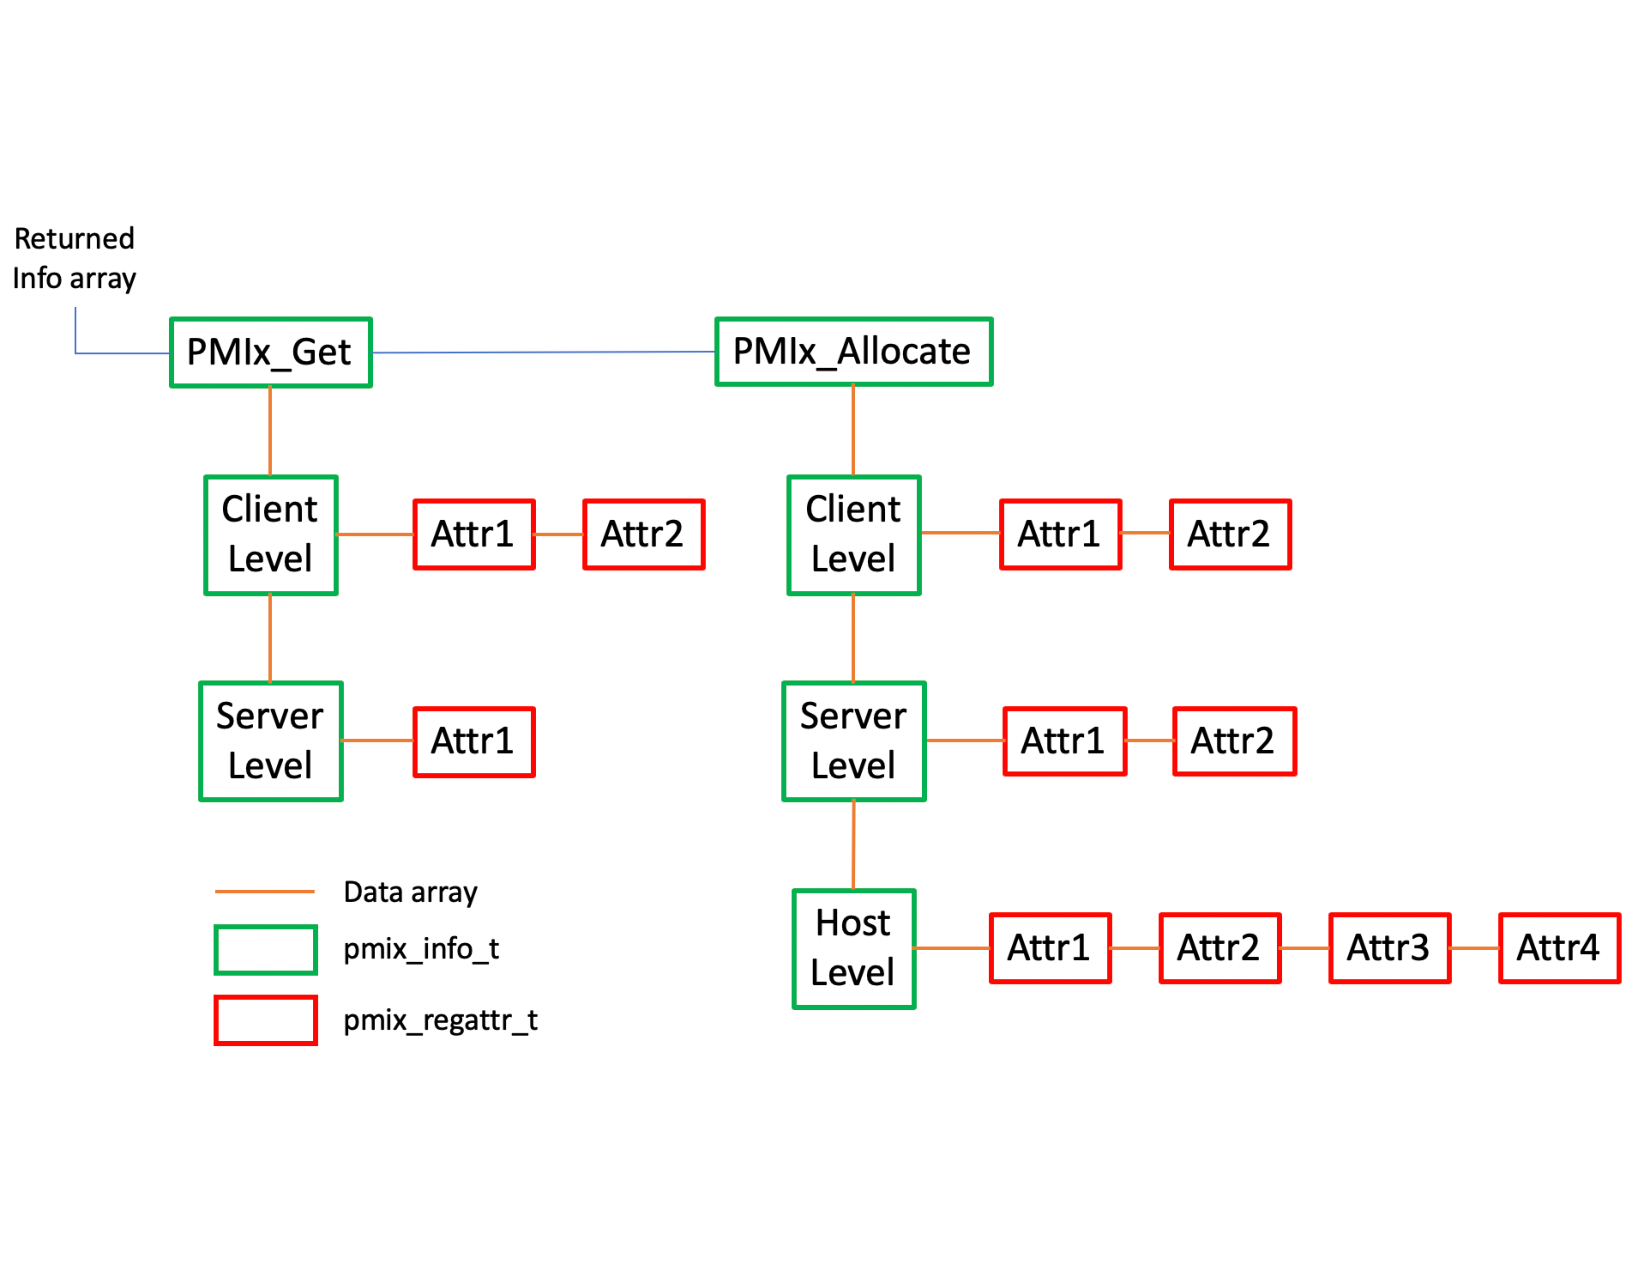
\includegraphics[clip,width=0.8\textwidth]{figs/attrquery.pdf}
  \end{center}
  \caption{Returned information hierarchy for attribute support request}
  \label{fig:attrquery}
\end{figure*}
\endgroup

The array of returned structures, and their child arrays, are subject to the return rules for the \refapi{PMIx_Query_info_nb} \ac{API}. For example, a request for supported attributes of the \refapi{PMIx_Get} function that includes the \refarg{host} level will return values for the \refarg{client} and \refarg{server} levels, plus an array element with a \refarg{key} of \refattr{PMIX_HOST_ATTRIBUTES} and a value type of \refconst{PMIX_UNDEF} indicating that no attributes are supported at that level.

%%%%%%%%%%%%%%%%%%%%%%%%%%%%%%%%%%%%%%%%%%%%%%%%%
